\section{Extended Evaluation}\label{sec:extended}

After the main study was complete and the method frozen, we ran a second, broader round of
tests designed to probe its weaknesses rather than its strengths. All constraint sets and
the CA-HRP-R scenario choice were fixed before any of these results were computed.

\subsection{External validation on three new universes}
We added three universes that played no role in any design decision: six Indian
exchange-traded funds (Nifty~50, Bank, Junior, PSU Bank, Nasdaq-100 and Gold BeES; April
2011 -- October 2026) under a balanced-fund mandate (gold $\le$ 25\%, international equity
$\le$ 35\%, Indian equity between 40\% and 80\%, single fund $\le$ 35\%); the ten US sector
SPDR funds (June 2000 -- October 2026), grouped as cyclical or defensive with defensive
sectors capped at 50\% and single sectors at 20\%; and nineteen single-country equity funds
(October 2004 -- October 2026) grouped into four regions, each capped at 40\% with single
countries at 10\%. Yahoo Finance records two short-lived unadjusted unit splits in the
Indian funds (December 2019 and June 2021), visible as $-90\%$ / $+900\%$ return pairs; we
detect such pairs automatically and rescale the affected prices by the implied split ratio
(10 or 100). No other universe is affected.

Table~\ref{tab:external} reports the results. Unconstrained HRP would breach these mandates
at 94\%, 92\% and 97\% of rebalances respectively, and HRP-Clip still breaches them at 1\%,
14\% and 9\%. CA-HRP is fully compliant. Its Sharpe ratio is above HRP-Proj in the Indian
(1.276 vs 1.257) and sector (0.628 vs 0.619) universes and slightly below it for countries
(0.428 vs 0.436), and in every universe it has the lowest volatility of the three HRP fixes.
Constrained minimum variance (Indian ETFs) and mean--variance (sectors) post the best Sharpe
ratios. The external evidence therefore confirms the pattern of the main study: CA-HRP is a
reliable way to make HRP compliant, with gains that scale with how hard the constraints
bind, but it does not dominate optimisation-based methods.

\begin{table*}[!htbp]\centering\small
\caption{External validation on three universes that were added after the method was frozen (net of 10\,bps). Vol and MaxDD in \%; Viol = share of rebalances breaching a constraint. Best constrained Sharpe ratio per universe in bold.}\label{tab:external}
\setlength{\tabcolsep}{4pt}\begin{tabular}{l rrrr rrrr rrrr}\toprule
 & \multicolumn{4}{c}{India ETFs} & \multicolumn{4}{c}{US sectors} & \multicolumn{4}{c}{Countries}\\
\cmidrule(lr){2-5}\cmidrule(lr){6-9}\cmidrule(lr){10-13}
Method & Sharpe & Vol & MaxDD & Viol & Sharpe & Vol & MaxDD & Viol & Sharpe & Vol & MaxDD & Viol\\\midrule
EW & 1.086 & 13.7 & -31.1 & 0\% & 0.586 & 18.3 & -55.2 & 0\% & 0.432 & 22.8 & -61.7 & 100\%\\
HRP & 1.336 & 10.5 & -21.5 & 94\% & 0.641 & 15.7 & -45.9 & 92\% & 0.427 & 21.1 & -59.5 & 97\%\\
\midrule
MinVar-C & \textbf{1.321} & 10.9 & -24.9 & 0\% & 0.653 & 15.7 & -48.1 & 0\% & 0.435 & 20.1 & -60.8 & 0\%\\
MVO-C & 1.052 & 14.5 & -28.1 & 0\% & \textbf{0.658} & 17.0 & -47.8 & 0\% & 0.386 & 22.1 & -64.8 & 0\%\\
HRP-Clip & 1.269 & 11.8 & -25.1 & 1\% & 0.613 & 16.6 & -49.1 & 14\% & 0.435 & 21.5 & -60.4 & 9\%\\
HRP-Proj & 1.257 & 11.9 & -25.6 & 0\% & 0.619 & 16.5 & -48.6 & 0\% & \textbf{0.436} & 21.5 & -60.1 & 0\%\\
CA-HRP-B & 1.255 & 11.9 & -25.2 & 0\% & 0.603 & 16.7 & -48.9 & 0\% & 0.412 & 21.6 & -61.0 & 0\%\\
\textbf{CA-HRP} & 1.276 & 11.3 & -24.9 & 0\% & 0.628 & 16.2 & -47.6 & 0\% & 0.428 & 21.2 & -60.0 & 0\%\\
CA-HRP-R & 1.275 & 11.3 & -25.6 & 0\% & 0.625 & 16.2 & -47.4 & 0\% & 0.426 & 21.2 & -60.1 & 0\%\\
\bottomrule\end{tabular}\end{table*}

\begin{figure}[!htbp]
\centering
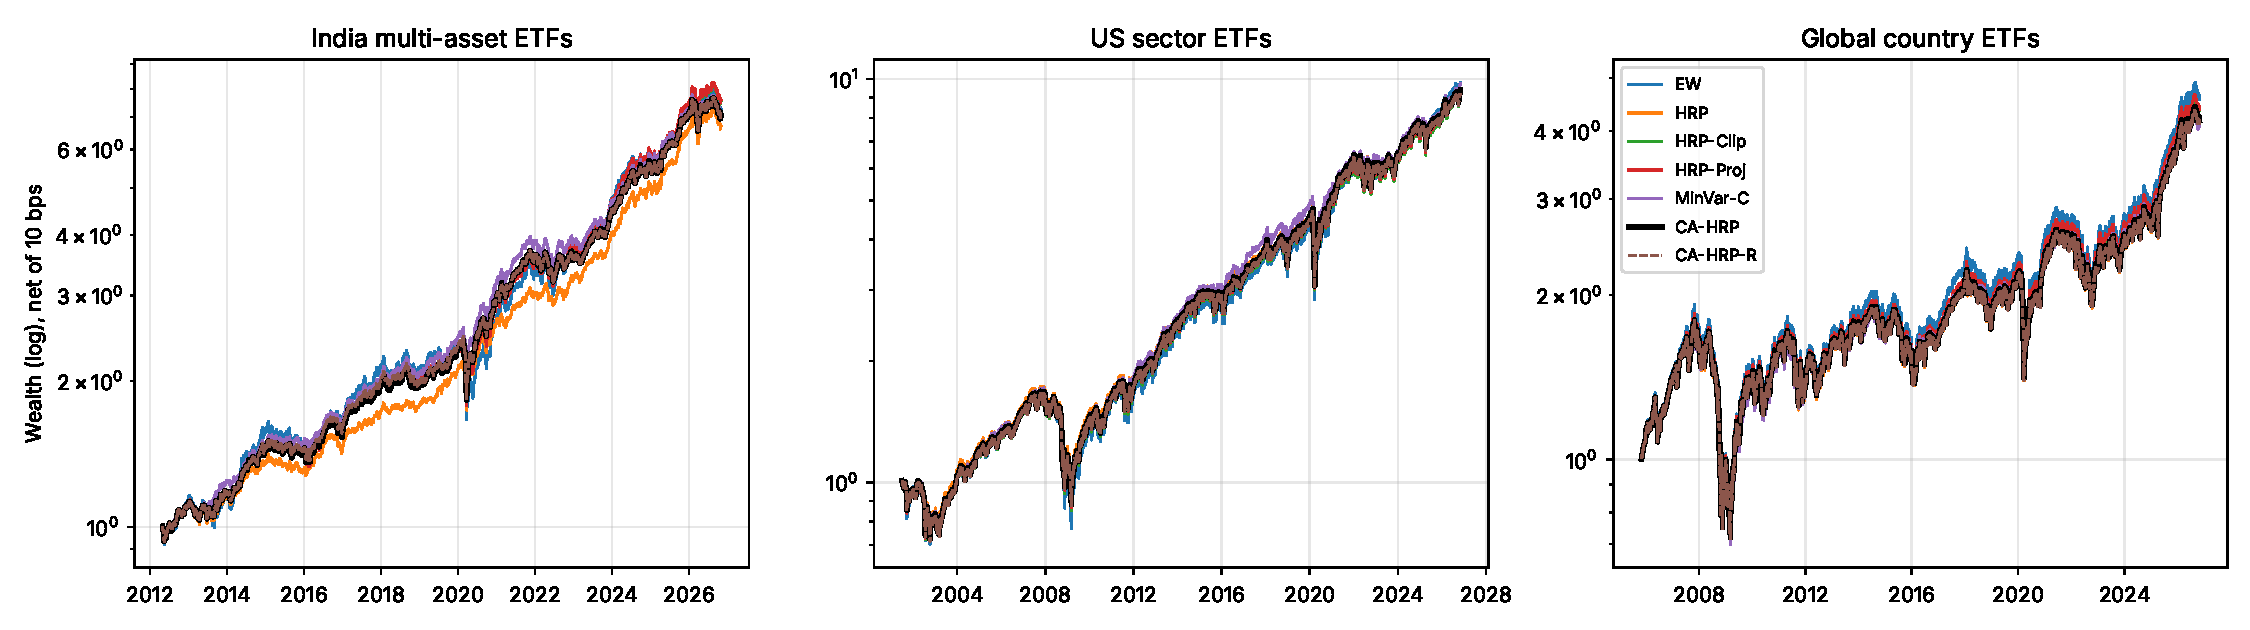
\includegraphics[width=\linewidth]{../results/figures/wealth_external.pdf}
\caption{Growth of one unit of wealth (log scale), net of 10\,bps, in the three external
universes.}
\label{fig:wealth-ext}
\end{figure}

\subsection{Statistical precision across six universes}
Table~\ref{tab:ci} and Figure~\ref{fig:ci} give bootstrap confidence intervals for the
Sharpe-ratio difference between CA-HRP and its competitors. Only one interval excludes
zero: CA-HRP versus HRP-Clip in the multi-asset ETF universe ($+0.20$, 95\% interval
$[+0.03,+0.35]$). The point estimate against HRP-Proj is positive in five of six universes
and is large only for multi-asset ETFs ($+0.145$, $[-0.04,+0.32]$). Against constrained
minimum variance it is negative in five of six universes but never significant. We
therefore claim reliability and lower risk, not superior returns.

\begin{table}[!htbp]\centering\small
\caption{Annualised Sharpe-ratio difference of CA-HRP minus each competitor, with 95\% circular-block-bootstrap intervals (21-day blocks, 2{,}000 draws). Intervals excluding zero in bold.}\label{tab:ci}
\resizebox{\linewidth}{!}{\begin{tabular}{lccccc}\toprule
Universe & HRP-Proj & HRP-Clip & MinVar-C & EW & CA-HRP-R\\\midrule
ETFs & +0.145 [-0.04, +0.32] & \textbf{+0.199 [+0.03, +0.35]} & -0.027 [-0.08, +0.03] & +0.146 [-0.04, +0.31] & +0.025 [-0.03, +0.08]\\
NIFTY & +0.001 [-0.03, +0.03] & +0.000 [-0.03, +0.03] & -0.032 [-0.15, +0.09] & +0.122 [-0.01, +0.25] & +0.002 [-0.00, +0.00]\\
US & +0.018 [-0.00, +0.04] & +0.018 [-0.00, +0.04] & +0.021 [-0.07, +0.11] & +0.027 [-0.08, +0.12] & +0.000 [-0.00, +0.00]\\
India ETFs & +0.019 [-0.07, +0.11] & +0.007 [-0.06, +0.07] & -0.045 [-0.14, +0.04] & +0.189 [-0.01, +0.38] & +0.001 [-0.03, +0.03]\\
US sectors & +0.010 [-0.01, +0.03] & +0.016 [-0.01, +0.04] & -0.024 [-0.08, +0.02] & +0.043 [-0.02, +0.11] & +0.003 [-0.00, +0.01]\\
Countries & -0.008 [-0.02, +0.01] & -0.007 [-0.02, +0.01] & -0.007 [-0.05, +0.03] & -0.004 [-0.04, +0.03] & +0.002 [-0.00, +0.01]\\
\bottomrule\end{tabular}}\end{table}

\begin{figure}[!htbp]
\centering
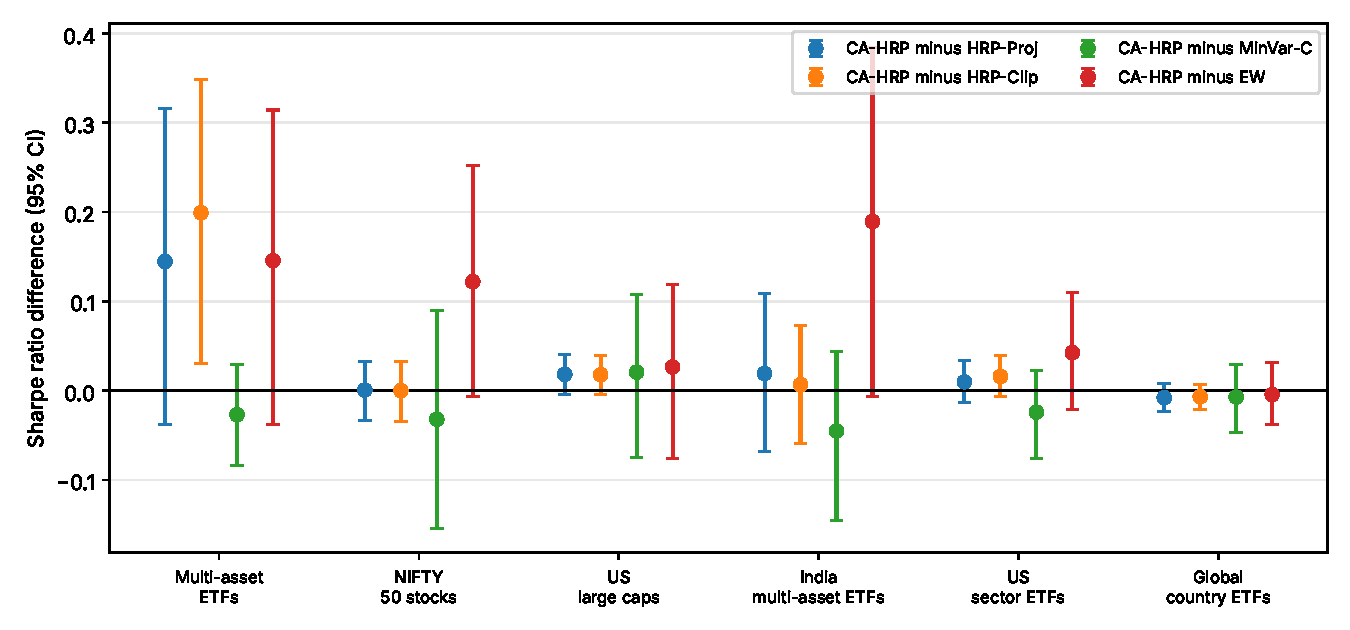
\includegraphics[width=0.85\linewidth]{../results/figures/sharpe_ci.pdf}
\caption{Sharpe-ratio difference of CA-HRP minus each competitor, with 95\% block-bootstrap
intervals, for all six universes.}
\label{fig:ci}
\end{figure}

\subsection{Does regime-robustness help?}
CA-HRP-R (Section~\ref{sec:robust}) was designed to address the 2022 weakness. It did not
help. Its Sharpe ratio is lower than CA-HRP's in all six universes, though never by more than
0.025, and it trades more (2.09 vs 1.25 annual turnover in the multi-asset universe).
In the 2022 rates shock it lost 18.1\% in the multi-asset universe against 17.2\% for CA-HRP.
The reason is visible in the validation study (Table~\ref{tab:robustdesign}): the only
scenario that would have anticipated 2022, the hedges-fail stress covariance, made the
portfolio much more conservative in normal times and was rejected on validation data.
Robustness to a regime that the estimation window has never seen cannot be bought cheaply
with covariance scenarios alone; we report this as a negative result.

\subsection{Rebalancing frequency}
Table~\ref{tab:freq} repeats the comparison with weekly and quarterly rebalancing (turnover
cap of 30\% per rebalance in both cases). CA-HRP satisfies all constraints at all
frequencies, while HRP-Clip breaches them at 9\% (weekly), 14\% (monthly) and 27\%
(quarterly) of rebalances on average across universes. Over the 18 frequency--universe
combinations, CA-HRP beats HRP-Proj in 12 and is the best HRP-based method in 10, while
constrained minimum variance beats CA-HRP in 16. The multi-asset ranking (CA-HRP clearly
ahead of the other HRP fixes, slightly behind minimum variance) holds at every frequency.

\begin{table*}[!htbp]\centering\small
\caption{Sharpe ratio by rebalancing frequency (W = weekly, M = monthly, Q = quarterly), net of 10\,bps, all six universes. The first column also gives HRP-Clip's share of rebalances with a constraint breach, pooled over universes (CA-HRP: 0\% at every frequency).}\label{tab:freq}
\setlength{\tabcolsep}{3.5pt}\begin{tabular}{ll rrrrrr}\toprule
Freq. & Universe & EW & MinVar-C & HRP-Clip & HRP-Proj & CA-HRP & CA-HRP-R\\\midrule
\multirow{6}{*}{\shortstack{W\\(Clip 9\%)}} & ETFs & 0.714 & 0.888 & 0.608 & 0.719 & \textbf{0.844} & 0.819\\
 & NIFTY & 1.268 & 1.414 & \textbf{1.329} & 1.328 & 1.326 & 1.325\\
 & US & 0.779 & 0.781 & \textbf{0.765} & 0.763 & 0.763 & 0.763\\
 & India ETFs & 1.066 & 1.331 & 1.258 & 1.241 & \textbf{1.269} & 1.261\\
 & US sectors & 0.588 & 0.655 & 0.600 & 0.609 & \textbf{0.612} & 0.609\\
 & Countries & 0.434 & 0.438 & 0.404 & \textbf{0.407} & 0.397 & 0.396\\
\midrule
\multirow{6}{*}{\shortstack{M\\(Clip 14\%)}} & ETFs & 0.763 & 0.935 & 0.709 & 0.764 & \textbf{0.908} & 0.884\\
 & NIFTY & 1.247 & 1.401 & 1.369 & 1.368 & \textbf{1.369} & 1.367\\
 & US & 0.767 & 0.773 & 0.775 & 0.775 & \textbf{0.793} & 0.793\\
 & India ETFs & 1.086 & 1.321 & 1.269 & 1.257 & \textbf{1.276} & 1.275\\
 & US sectors & 0.586 & 0.653 & 0.613 & 0.619 & \textbf{0.628} & 0.625\\
 & Countries & 0.432 & 0.435 & 0.435 & \textbf{0.436} & 0.428 & 0.426\\
\midrule
\multirow{6}{*}{\shortstack{Q\\(Clip 27\%)}} & ETFs & 0.807 & 0.920 & 0.719 & 0.800 & \textbf{0.899} & 0.873\\
 & NIFTY & 1.233 & 1.375 & 1.357 & 1.354 & 1.361 & \textbf{1.361}\\
 & US & 0.787 & 0.744 & \textbf{0.812} & 0.808 & 0.807 & 0.808\\
 & India ETFs & 1.107 & 1.317 & 1.279 & 1.261 & 1.295 & \textbf{1.299}\\
 & US sectors & 0.593 & 0.643 & 0.620 & 0.625 & \textbf{0.634} & 0.631\\
 & Countries & 0.415 & 0.416 & 0.421 & \textbf{0.423} & 0.409 & 0.409\\
\bottomrule
\end{tabular}\end{table*}

\subsection{Which constraints matter?}
Table~\ref{tab:decomp} imposes the constraint families one at a time. In the multi-asset
universe almost all of CA-HRP's advantage comes from the \emph{group} constraints: with
group caps and floors alone its Sharpe ratio is 0.972 against 0.745 for HRP-Proj and 0.684
for HRP-Clip, whereas with per-asset caps alone the gap is much smaller (0.853 vs 0.802).
This is consistent with Proposition~\ref{prop:te}(d): group caps remove a large block of
correlated weight at once, which is exactly where choosing replacements by covariance
rather than uniformly pays off. With per-asset caps alone in the Indian ETF universe,
CA-HRP is slightly worse than the simple fixes (1.300 vs 1.312--1.314). HRP-Clip never breaches
per-asset caps on their own; its breaches come from group caps and floors (36\% of
rebalances with groups alone in the multi-asset universe) and, in the sector universe, only
from the turnover budget that it ignores.

\begin{table}[!htbp]\centering\small
\caption{Which constraints matter? Sharpe ratio (net of 10\,bps) when only some constraint families are imposed. Best HRP-family method per row in bold.}\label{tab:decomp}
\setlength{\tabcolsep}{4pt}\begin{tabular}{ll rrr}\toprule
Universe & Constraints & HRP-Clip & HRP-Proj & CA-HRP\\\midrule
\multirow{4}{*}{ETFs} & box only & 0.777 & 0.802 & \textbf{0.853}\\
 & groups only & 0.684 & 0.745 & \textbf{0.972}\\
 & box + groups & 0.709 & 0.764 & \textbf{0.910}\\
 & all (+ turnover) & 0.709 & 0.764 & \textbf{0.908}\\
\midrule
\multirow{4}{*}{India ETFs} & box only & \textbf{1.314} & 1.312 & 1.300\\
 & groups only & 1.269 & 1.257 & \textbf{1.273}\\
 & box + groups & 1.269 & 1.257 & \textbf{1.273}\\
 & all (+ turnover) & 1.269 & 1.257 & \textbf{1.276}\\
\midrule
\multirow{4}{*}{US sectors} & box only & 0.614 & 0.612 & \textbf{0.628}\\
 & groups only & 0.626 & 0.635 & \textbf{0.639}\\
 & box + groups & 0.613 & 0.620 & \textbf{0.628}\\
 & all (+ turnover) & 0.613 & 0.619 & \textbf{0.628}\\
\midrule
\multirow{4}{*}{US} & box only & 0.775 & 0.774 & \textbf{0.792}\\
 & groups only & 0.777 & 0.776 & \textbf{0.795}\\
 & box + groups & 0.775 & 0.774 & \textbf{0.793}\\
 & all (+ turnover) & 0.775 & 0.775 & \textbf{0.793}\\
\bottomrule
\end{tabular}\end{table}

\subsection{Monte Carlo evidence with a known covariance}
Backtests mix estimation error with luck. To isolate the former we simulate 40 assets in
five correlated clusters, one of which is a low-volatility, negatively correlated ``bond''
block, so that HRP on the \emph{true} covariance puts 90\% in that block and breaches a
per-asset cap of $2.5/N$ and group caps of 30\%. Groups coincide with clusters except for two
assets per cluster, so constraints cut across the tree. Every asset has an annualised Sharpe
ratio of 0.4. For each of 200 replications per cell we draw $T\in\{126,252,504\}$ daily
returns (Gaussian or Student-$t_5$), estimate each method, and evaluate the resulting
portfolio under the true parameters.

Table~\ref{tab:mc} and Figure~\ref{fig:mc} show the Student-$t$ case (the Gaussian case is
almost identical). CA-HRP has the highest true Sharpe ratio of all methods in every cell
(0.809--0.820 under fat tails, 0.813--0.822 under normality). Among the HRP-based methods it
has the lowest true tracking error to the oracle HRP portfolio (6.0--6.3\%, against
7.3--7.4\% for HRP-Clip and 8.2\% for HRP-Proj), on par with constrained minimum variance
(within 0.05 percentage points). Its true volatility also matches constrained minimum
variance (6.4--6.7\%), while HRP-Proj is 8.5\% and constrained mean--variance
13.7--14.3\%. The cross-replication standard
deviation of the true Sharpe ratio is below 0.01, so these differences are precisely
estimated. In this controlled setting, which isolates the constraint-handling problem the
paper is about, CA-HRP is the best method.

\begin{table*}[!htbp]\centering\small
\caption{Monte Carlo study with a known covariance (40 assets, 5 clusters, 200 replications per cell). True Sharpe ratio and true volatility (\%) of the estimated portfolio, and true tracking error (\%) to HRP computed on the true covariance. Best value per column among constrained methods in bold.}\label{tab:mc}
\setlength{\tabcolsep}{4pt}\begin{tabular}{l rrr rrr rrr}\toprule
 & \multicolumn{3}{c}{True Sharpe ratio} & \multicolumn{3}{c}{True volatility} & \multicolumn{3}{c}{True TE to true HRP}\\
\cmidrule(lr){2-4}\cmidrule(lr){5-7}\cmidrule(lr){8-10}
Method (Student-$t_5$) & $T$=126 & 252 & 504 & 126 & 252 & 504 & 126 & 252 & 504\\\midrule
EW & 0.722 & 0.722 & 0.722 & 12.62 & 12.62 & 12.62 & 12.49 & 12.49 & 12.49\\
MVO-C & 0.680 & 0.683 & 0.684 & 14.00 & 13.80 & 13.86 & 13.85 & 13.65 & 13.71\\
MinVar-C & 0.808 & 0.809 & 0.811 & \textbf{6.63} & \textbf{6.52} & 6.44 & \textbf{6.28} & 6.17 & 6.09\\
HRP-Clip & 0.806 & 0.806 & 0.808 & 7.74 & 7.74 & 7.72 & 7.39 & 7.39 & 7.37\\
HRP-Proj & 0.804 & 0.804 & 0.804 & 8.53 & 8.54 & 8.52 & 8.18 & 8.20 & 8.18\\
\textbf{CA-HRP} & \textbf{0.809} & \textbf{0.813} & \textbf{0.820} & 6.66 & 6.52 & \textbf{6.43} & 6.32 & \textbf{6.17} & \textbf{6.04}\\
CA-HRP-R & 0.808 & 0.808 & 0.811 & 6.73 & 6.64 & 6.57 & 6.39 & 6.31 & 6.22\\
\bottomrule\end{tabular}\end{table*}

\begin{figure}[!htbp]
\centering
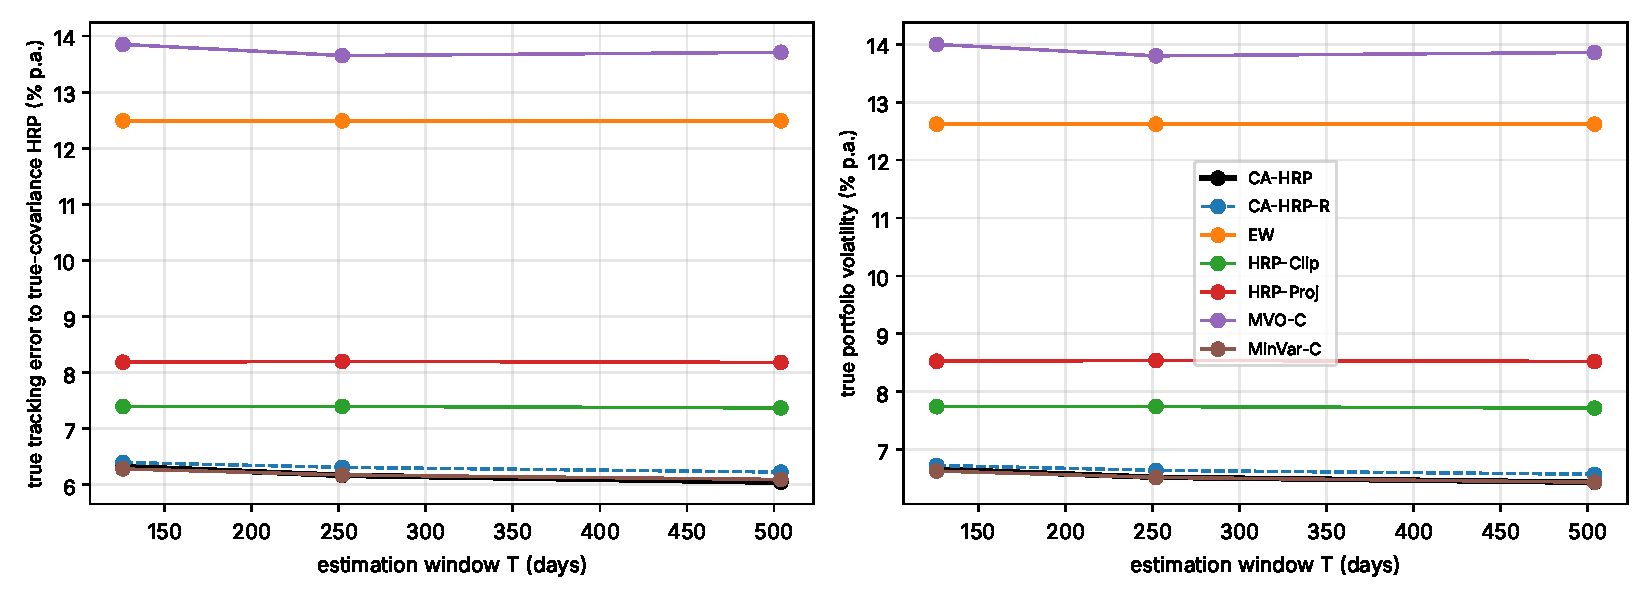
\includegraphics[width=0.9\linewidth]{../results/figures/montecarlo.pdf}
\caption{Monte Carlo (Student-$t_5$): true tracking error to the oracle HRP portfolio and
true volatility as a function of the estimation window.}
\label{fig:mc}
\end{figure}

\subsection{Computational cost}
Figure~\ref{fig:runtime} reports the median time per rebalance for random universes of
$N=10$ to $400$ assets with ten groups and a turnover cap. CA-HRP takes 17\,ms at $N=50$ and
0.27\,s at $N=400$, the same order as constrained minimum variance (0.25\,s). The
solver-free CA-HRP-B takes 0.15\,s at $N=400$ and the regime-robust CA-HRP-R 1.4\,s, so the
robust variant is the only one whose cost grows noticeably. All are negligible for monthly
rebalancing.

\begin{figure}[!htbp]
\centering
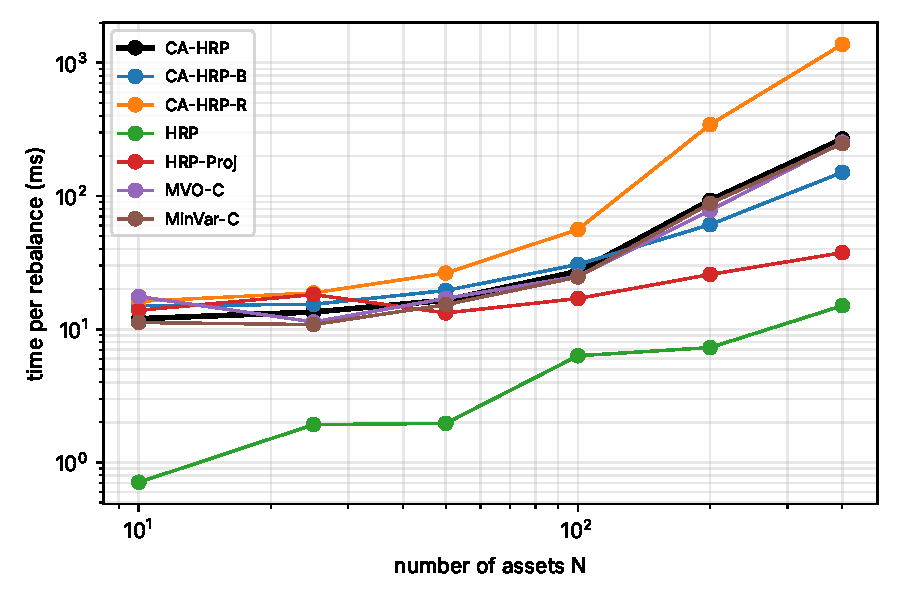
\includegraphics[width=0.55\linewidth]{../results/figures/runtime.pdf}
\caption{Median computation time per rebalance against the number of assets (log--log).}
\label{fig:runtime}
\end{figure}
